\documentclass[tikz,border=2pt]{standalone}
% Preámbulo común de los diagramas TikZ (misma paleta y letra que las notas)
\usepackage[T1]{fontenc}\usepackage[utf8]{inputenc}
\usepackage{libertinus}\usepackage{libertinust1math}
\usepackage[defaultsans,scale=0.92]{lato}
\usepackage{amsmath,amssymb,bm}
\usepackage{tikz}\usetikzlibrary{calc,positioning,arrows.meta,shapes.geometric,decorations.pathreplacing,decorations.pathmorphing,fit,backgrounds}
\definecolor{snlazul}{HTML}{1E5AA8}\definecolor{snlnoche}{HTML}{14213D}\definecolor{snlvioleta}{HTML}{6C4AB6}
\definecolor{snlcoral}{HTML}{D1495B}\definecolor{snlambar}{HTML}{E09F3E}\definecolor{snlverde}{HTML}{2A9D8F}
\definecolor{snlteal}{HTML}{0F7173}\definecolor{snlgris}{HTML}{5C677D}\definecolor{snlfondo}{HTML}{F4F6FA}
\tikzset{>={Stealth[length=2.2mm]},
  bloque/.style={draw=#1,fill=#1!8,thick,rounded corners=2pt,minimum height=11mm,minimum width=20mm,align=center,font=\small},
  bloque/.default=snlazul,
  suma/.style={draw=snlnoche,thick,circle,inner sep=0pt,minimum size=5mm},
  flecha/.style={->,thick,draw=snlnoche},
  etq/.style={font=\small,text=snlnoche},
  nota/.style={font=\footnotesize\sffamily,text=snlgris,align=center}}

\begin{document}
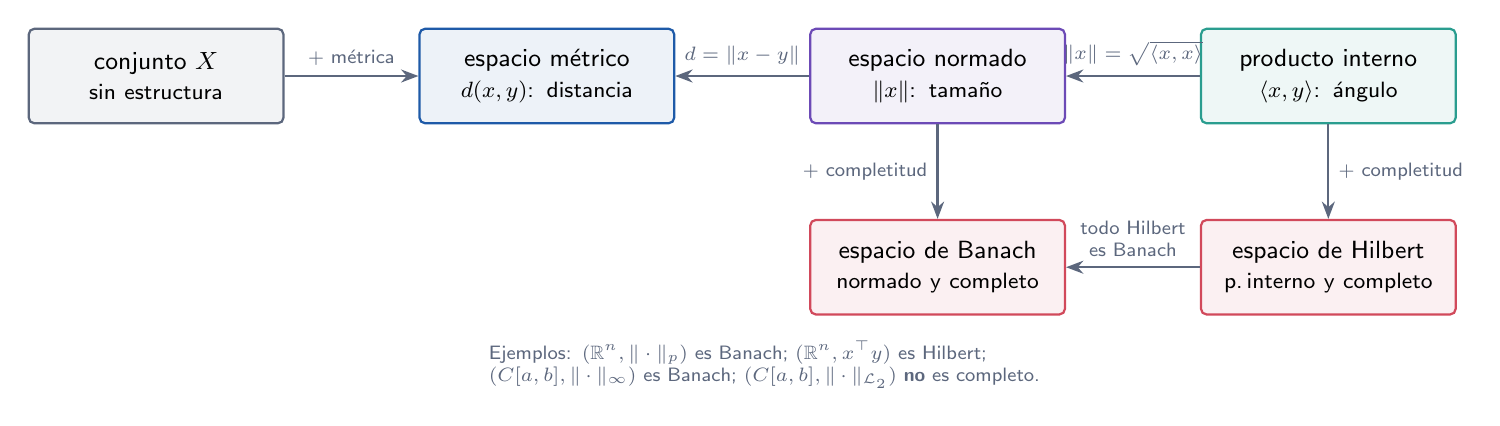
\begin{tikzpicture}[font=\sffamily\small,
  caja/.style={draw=#1,fill=#1!8,thick,rounded corners=2pt,align=center,minimum height=12mm,text width=30mm},
  fl/.style={-{Stealth[length=2.2mm]},thick,draw=snlgris},
  et/.style={font=\sffamily\scriptsize,text=snlgris,align=center}]
  \node[caja=snlgris] (con) {conjunto $X$\\ \footnotesize sin estructura};
  \node[caja=snlazul,right=17mm of con] (met) {espacio métrico\\ \footnotesize $d(x,y)$: distancia};
  \node[caja=snlvioleta,right=17mm of met] (nor) {espacio normado\\ \footnotesize $\|x\|$: tamaño};
  \node[caja=snlverde,right=17mm of nor] (pi) {producto interno\\ \footnotesize $\langle x,y\rangle$: ángulo};
  \node[caja=snlcoral,below=12mm of nor] (ban) {espacio de Banach\\ \footnotesize normado y completo};
  \node[caja=snlcoral,below=12mm of pi] (hil) {espacio de Hilbert\\ \footnotesize p.\,interno y completo};
  \draw[fl] (con) -- node[et,above]{+ métrica} (met);
  \draw[fl] (nor) -- node[et,above]{$d=\|x-y\|$} (met);
  \draw[fl] (pi) -- node[et,above]{$\|x\|=\sqrt{\langle x,x\rangle}$} (nor);
  \draw[fl] (nor) -- node[et,left]{+ completitud} (ban);
  \draw[fl] (pi) -- node[et,right]{+ completitud} (hil);
  \draw[fl] (hil) -- node[et,above]{todo Hilbert\\es Banach} (ban);
  \node[et,below=2mm of ban,xshift=-22mm,text width=70mm,align=left] {Ejemplos: $(\mathbb{R}^n,\|\cdot\|_p)$ es Banach; $(\mathbb{R}^n,x^\top y)$ es Hilbert;\\
     $(C[a,b],\|\cdot\|_\infty)$ es Banach; $(C[a,b],\|\cdot\|_{\mathcal{L}_2})$ \textbf{no} es completo.};
\end{tikzpicture}
\end{document}
